\documentclass[titlepage, a4paper, 12pt, reqno, openany]{report}
%\documentclass[12pt]{report}
%\documentclass[titlepage, a4paper, 12pt, reqno, openany]{article}
%\documentclass[12pt]{article}
%%%%%%%%%%%%%%%%%%%%%%%%%%%%%%%%%%%%%%%%%%%%%%%%%%%%%%%%%%%%%%%%%%%%%%%%%%%%%
\usepackage{titlepic}
%%%%%%encoding%%%%%%
\usepackage[T1]{fontenc}
\usepackage[utf8]{inputenc}
\usepackage{hyphenat}
\usepackage[portuguese]{babel}
%%%%%%Hyphenation rules%%%%%%
\usepackage{graphicx} %permite inserir figuras
\usepackage[font=small,labelfont=bf]{caption} %reference figures
%\usepackage{subcaption}
\usepackage{color,colortbl,multirow}
\usepackage[top=2cm,left=1cm,right=1cm,bottom=2cm]{geometry}
%\usepackage[margin=2cm]{geometry} %margens
%\usepackage[left=2cm,top=1cm,bottom=2cm,right=3cm,nohead,nofoot]{geometry}
\usepackage{paralist}
\usepackage{float}
\usepackage{verbatim}
\usepackage{lipsum}
\usepackage{multicol}
\usepackage{babelbib}
\usepackage{amsfonts}
\usepackage{amsmath}
\usepackage{amssymb}
%%%%%%%%%%%%%%%%%%%%%%%%%%%%%%%%%%%%%%%%%%%%%%%%%%%%%%%%%%%%%%%%%%%%%%%%%%%%%%%
\usepackage[usenames,dvipsnames,svgnames,table]{xcolor} %\usepackage[usenames]{color} %permite letras coloridas
\usepackage{adjustbox}
\usepackage{makecell}
%\usepackage{times}
%\usepackage{makeidx} %para criar índice remissivo
%\usepackage{array}
%\usepackage{supertabular}
%\usepackage{bm}
%\usepackage{booktabs}
%\usepackage{boxedminipage}
%\usepackage{caption}
%\usepackage{changepage}
%\usepackage{cite}
%\usepackage{easylist}
%\usepackage{esint}
%\usepackage{eucal}
%\usepackage{fancyhdr}
%\usepackage{hyperref} %index dentro de red boxes
%\usepackage{indentfirst}
%\usepackage{latexsym}
%\usepackage{listings}
%\usepackage{mathptmx}
%\usepackage{mathrsfs} %permite o uso de letras trabalhadas
%\usepackage{microtype}
%\usepackage[normalem]{ulem} %permite sublinhar palavras
%\usepackage{pifont}
%\usepackage{rotating}
%\usepackage{setspace}
%\usepackage{syntonly} %speedup work desabling pdf converse \syntaxonly
%\usepackage{subfiles}
%\usepackage{textcomp}
%\usepackage{theorem}
%\usepackage{ulem}
%\usepackage{url}
%\usepackage{wrapfig}
%%%%%recent%%%%%
%\usepackage{cancel}
%\usepackage[fleqn]{mathtools}
%\usepackage{pdfpages}
%\usepackage{pdflscape}
%\usepackage{todonotes}
%\usepackage{siunitx}
%%%%%%%%%%%%%%%%%%%%%%%%%%%%%%%%%%%%%%%%%%%%%%%%%%%%%%%%%%%%%%%%%%%%%%%%%%%%%%%%%%%
%\renewcommand\thesection{\arabic{section}}
%\renewcommand\thesubsection{\thesection.\arabic{subsection}}
%%%%%%%%%%%%%%%%%%%%%%%%%%%%%%%%%%%%%%%%%%%%%%%%%%%%%%%%%%%%%%%%%%%%%%%%%%%%%%%%%%%%
\begin{comment}
\usepackage{enumitem}
\setlistdepth{12}
\newlist{enumitem}{enumerate}{12}
\setlist[enumitem,1]{label=\roman*)}
\setlist[enumitem,2]{label=\alph*)}
\setlist[enumitem,3]{label=\arabic*)}
\setlist[enumitem,4]{label=(\roman*)}
\setlist[enumitem,5]{label=(\alph*)}
\setlist[enumitem,6]{label=(\arabic*)}
\setlist[enumitem,7]{label=\roman*)}
\setlist[enumitem,8]{label=\alph*)}
\setlist[enumitem,9]{label=\arabic*)}
\setlist[enumitem,10]{label=(\roman*)}
\setlist[enumitem,11]{label=(\alph*)}
\setlist[enumitem,12]{label=(\arabic*)}
\end{comment}

%%%%%%%%%%%%%%%%%%%%%%%%%%%%%%%%%%%%%%%%%%%%%%%%%%%%%%%%%%%%%%%%%%%%%%%%%%%%%%%%%%%%
\begin{comment}
\usepackage{enumerate}
\renewcommand{\labelitemi}{$\bullet$}
\renewcommand{\labelitemii}{$\cdot$}
\renewcommand{\labelitemiii}{$\diamond$}
\renewcommand{\labelitemiv}{$\ast$}
\end{comment}

%%%%%%%%%%%%%%%%%%%%%%%%%%%%%%%%%%%%%%%%%%%%%%%%%%%%%%%%%%%%%%%%%%%%%%%%%%%%%%%%%%%%
\begin{comment}
\usepackage{tikz}
\usepackage{circuitikz}
\usetikzlibrary{matrix,shapes.geometric,arrows,trees,positioning,calc}
%%%%%%%%%%%%%%%%%%%%%%%pre defined figures%%%%%%%%%%%%%%%%%%%%%
\tikzstyle{RECTANGLE_2} = [rectangle, draw, text width=5em, text centered, rounded corners, minimum height=4em]
\tikzstyle{RECTANGLE_3} = [rectangle, rounded corners, minimum width=3cm, minimum height=1cm,text centered, draw=black, fill=red!80]
\tikzstyle{RECTANGLE_4} = [rectangle, draw, fill=blue!20, text width=3cm, text centered, minimum height=4em]
\tikzstyle{RECTANGLE_5} = [rectangle, minimum width=3cm, minimum height=1cm, text centered, text width=3cm]
\tikzstyle{RECTANGLE_6} = [rectangle, draw, fill=blue!20, text width=5em, text centered, rounded corners, minimum height=4em]
\tikzstyle{RECTANGLE_7} = [rectangle, draw, fill=blue!20, text width=5em, text centered, rounded corners, minimum height=4em]
\tikzstyle{RECTANGLE_8} = [rectangle, draw, align=left, fill=blue!20]
\tikzstyle{RECTANGLE_1} = [rectangle, rounded corners, minimum width=1cm, minimum height=1cm,text centered, draw=black, fill=green!%30]
\tikzstyle{DIAMOND_1} = [diamond, draw, fill=blue!20, text width=4.5em, text badly centered, node distance=4cm, inner sep=0pt]
\tikzstyle{DIAMOND_2} = [diamond, minimum width=3cm, minimum height=1cm, text centered, draw=black, fill=green!30]
\tikzstyle{DIAMOND_3} = [diamond, draw, text width=4.5em, text badly centered, node distance=3cm, inner sep=0pt]
\tikzstyle{DIAMOND_4} = [diamond, draw, fill=blue!20, text width=4.5em, text badly centered, node distance=3cm, inner sep=0pt]
\tikzstyle{DIAMOND_5} = [diamond, draw, fill=blue!20, text width=4.5em, text badly centered, node distance=3cm, inner sep=0pt]
\tikzstyle{DIAMOND_6} = [diamond, draw, fill=blue!20, text width=4.5em, text badly centered, node distance=4cm, inner sep=0pt]
\tikzstyle{DIAMOND_7} = [diamond, draw, align=left, fill=blue!20]
\tikzstyle{ELLIPSE_1} = [draw, ellipse,fill=red!20, node distance=3cm, minimum height=2em]
\tikzstyle{ELLIPSE_2} = [draw, ellipse,fill=red!20, node distance=3cm, minimum height=2em]
\tikzstyle{ELLIPSE} = [draw, ellipse,fill=red!20, node distance=3cm, minimum height=2em]
\tikzstyle{TRAPEZIUM_1} = [trapezium,trapezium left angle=70,trapezium right angle=-70,minimum height=0.6cm, draw, fill=blue!20, text width=4.5em, text badly centered, node distance=3cm, inner sep=0pt]
\tikzstyle{TRAPEZIUM_2} = [trapezium, trapezium left angle=70, trapezium right angle=110, minimum width=3cm, minimum height=1cm, text centered, draw=black, fill=blue!30]
\tikzstyle{TRAPEZIUM_3} = [trapezium,trapezium left angle=70,trapezium right angle=-70,minimum height=0.6cm, draw, fill=blue!20, text width=4.5em, text badly centered, node distance=3cm, inner sep=0pt]
\tikzstyle{ARROW} = [thick,->,>=stealth]
\tikzstyle{LINE} = [draw, -latex']
\tikzstyle{MYLINE} = [draw, ->,  thick, shorten <=4pt, shorten >=4pt]
\tikzstyle{TEXT_1}=[draw,text centered,minimum size=6em,text width=5.25cm,text height=0.34cm]
\tikzstyle{TEXT_2}=[draw,text centered,minimum size=2em,text width=2.75cm,text height=0.34cm]
\tikzstyle{TEXT_3}=[draw,minimum size=2.5em,text centered,text width=3.5cm]
\tikzstyle{TEXT_4}=[draw,minimum size=3em,text centered,text width=6.cm]
\tikzstyle{CIRCLE_1}=[draw,shape=circle,inner sep=2pt,text centered, node distance=3.5cm]
\tikzstyle{CIRCLE_2}=[draw,shape=circle,inner sep=4pt,text centered, node distance=3.cm]
\end{comment}

%%%%%%%%%%%%%%%%%%%%%%%%%%%%%%%%%Not Adviced%%%%%%%%%%%%%%%%%%%%%%%%%%%%%%%%%%%%%%%%
%\usepackage{showidx} %for troubleshooting index
%\usepackage{showkeys} %for troubleshooting \label \ref
%\usepackage{pxfonts}

%%%%%%%%%%%%%%%%%%%%%%%%%%%%%%%%%claching Package%%%%%%%%%%%%%%%%%%%%%%%%%%%%%%%%%%%
%\usepackage{pgfplots}
%\usepackage{natbib}
%\usepackage[usenames]{color} %permite letras coloridas
%\usepackage{xypic}

%%%%%%%%%%%%%%%%%%%%%%%%%%%%%%%%%Not Installed Yet%%%%%%%%%%%%%%%%%%%%%%%%%%%%%%%%%%

%%%%%%%%%%%%%%%%%%%%%%%%%%%%%%%Com Dependencias%%%%%%%%%%%%%%%%%%%%%%%%%%%%%%%%%%%%%
%\usepackage{glossaries}
%\usepackage[version=3]{mhchem}

%%%%%%%%%%%%%%%%%%%%%%%%%%%%%%%%%%%%%%%%%%%%%%%%%%%%%%%%%%%%%%%%%%%%%%%%%%%%%%%%%%%%
% alguns pacotes nao sao reconhecidos, ter atencao quais usar em differents computadores, tambem alguns pacotes entram em conflito.
\newtheorem{theorem}{Theorem}
\newtheorem{lemma}{Lemma}
\newtheorem{definition}{Defini\c{c}\~{a}o}
\newtheorem{notation}{Notation}

%%%%%%%%%%%%%%%%%%%%%%%%%%%%%%%%Not Working%%%%%%%%%%%%%%%%%%%%%%%%%%%%%%%%%%%%%%%%%
%\usepackage{itemize}
%\usepackage{named}
%\usepackage{amscls}
%\usepackage{fullpage}

%%%%%%%%%%%%%%%%%%%%%%%%%%%%%%%%%%%%%%%%%%%%%%%%%%%%%%%%%%%%%%%%%%%%%%%%%%%%%%%%%%%%
%\usepackage{apacite} %Bibliography style
%%%%%%%%%%%%%%%%%%%%%%%%%%%%%%%%%%%%%%%%%%%%%%%%%%%%%%%%%%%%%%%%%%%%%%%%%%%%%%%%%%%%
\makeindex
%%%%%%%%%%%%%%%%%%%%%%%%%%%%%%%%%%%%%%%%%%%%%%%%%%%%%%%%%%%%%%%%%%%%%%%%%%%%%%%%%%%%
\begin{document}
%\bibliographystyle{apacite}
\bibliographystyle{babplain}
%%%%%%%%%%%%%%%%%%%%%%%%FIX SECTION NUMBERING IN CASE REPORT%%%%%%%%%%%%%%%%%%%%%%%%
\renewcommand\thesection{\arabic{section}}
\renewcommand\thesubsection{\thesection.\arabic{subsection}}
\renewcommand\thesubsubsection{\thesection.\thesubsection.\arabic{subsubsection}}

\begin{minipage}{\linewidth}

\title{Comportamento Organizacional}
\author{
\emph{S\'{e}rgio Santos},\;$N^o$:\; 1020881 \\
\emph{Nome 2},\;$N^o$:\; 2000000\\
\emph{Nome 3},\;$N^o$:\; 3000000\\
%\emph{Nome 4},\;$N^o$:\; 4000000\\
%\emph{Nome 5},\;$N^o$:\; 5000000\\
}
\date{\today}
%\titlepic{
\includegraphics[scale=0.50]{./image/ROQ/ROQ.jpg}}

\begin{titlepage}

\includegraphics[scale=0.60]{./image/capa/ISEP_marca_cor_grande.png}
\maketitle
\vspace{8cm}
\begin{flushleft}

\includegraphics[scale=0.50]{./image/ROQ/ROQ.jpg}
\end{flushleft}
\end{titlepage}

\end{minipage}

\tableofcontents
\appendix
\pagestyle{plain} %plain headings empty
%\setcounter{chapter}{0}
%\numberwithin{page}{section}
%\renewcommand{\abstractname}{Executive Summary}
\captionsetup{justification = raggedright, singlelinecheck = false}
\setlength{\parindent}{0in}
%%%%%%%%%%%%%%%%%%%%%%%%%%%%%%%%%%%%%%%%%%%%%%%%%%%%%%%%%%%%%%%%%%%%%%%%%%%%%%%%%%%%%%%%%%%%%%%%%%%%%%%%%%%%%%%
\label{Resumo}
\begin{abstract}
\qquad Este trabalho vai abordar os assuntos mencionados no titulo, primeiro vai ser classificado as classes de trabalhador e uma breve explicação e comparação simples das mais comum na nossa sociedade o trabalhador por conta de outrem e o independente, uma breve descrição das novas tendências no mercado de trabalho que estão a surgir, também mostrar a importância da gestão da carreira individual e formas de a valorizar.\\
\\
Vai ser também abordado a importância da mudanças com a entrada das novas tecnologias no ambiente de trabalho, um estudo das competências e a valorização pessoal.\\
\\
A matéria relacionada com esta disciplina estará sempre presente nos assuntos abordados.\\
\vfill
\textbf{Palavras Chave:} Mudança, Liderança, Gestão de Equipas
\end{abstract}
%%%%%%%%%%%%%%%%%%%%%%%%%%%%%%%%%%%%%%%%%%%%%%%%%%%%%%%%%%%%%%%%%
\newpage
\section{Introdução}
%%%%%%%%%%%%%%%%%%%%%%%%%%%%%%%%%%%%%%%%%%%%%%%%%%%%%%%%%%%%%%%%%
\qquad A juventude foi ensinada que a missão de se tornarem adultos, o caminho de dignidade, segurança e independência é obter um emprego.\cite{book_11}\\
O estágio uma ferramenta muito importante para qualquer iniciante de qualquer profissão de forma a ser transmitido conhecimentos adquiridos, que em certas profissões pode demorar até alguns anos para alcançar a categoria de oficial ou sénior.\\
\\
O cidadão deve estar numa das situações contributiva abaixo descrito para ser considerado um trabalhador em regime legal.\\
\\
\begin{minipage}[t]{\linewidth}
\begin{itemize}
\setlength\itemsep{-0.3em}
\item Trabalhador por conta de outrem
\begin{itemize}
\item Organização privada
\item Organização pública
\end{itemize}
\item Trabalhadores independentes
\begin{itemize}
\item Recibos Verdes
\item Falsos Recibos Verdes
\item subcontratado
\end{itemize}
\newpage
\item Trabalhador do serviço domestico
\item Membros de órgãos estatuários
\item Empresa
\item Político\\ \\
\end{itemize}
\end{minipage}
\subsection{trabalhador por conta de outrem}
\begin{figure}[H]
%\centering
\flushleft
%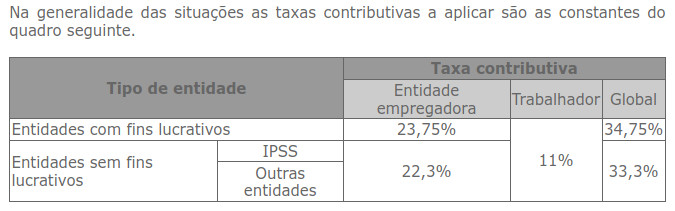
\includegraphics[width=.6\textwidth,left]{./image/SGS/Contribuicoes_1.jpg}
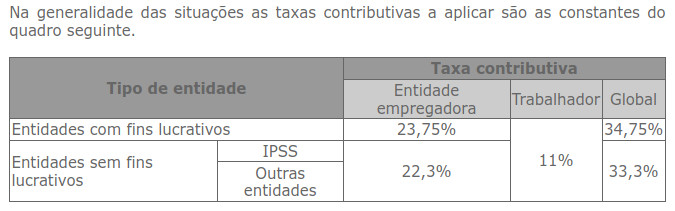
\includegraphics[scale=.5]{./image/SGS/Contribuicoes_1.jpg}
\caption{Contribuições para SGS}
\end{figure}\par
\qquad Como podemos ver o cidadão desconta, 34,5\% e 33,3\% respetivamente para o estado.\\
Exemplo:\\ 
Vencimento de 1000Eur será descontado 11\% para a Segurança Social, ficando com $1000\times (1-0,11)=890Eur$ e a empresa desconta para o exemplo de 23,75\%, $1000\times 0,2375=237,5Eur$, ao todo será descontado $110+237,5=347,5Eur$, ou seja, todos os messes um trabalhador que ganhe 1000Eur desconta para a Segurança Social direto e indiretamente \textbf{347,5Eur}.\\ \\
Na realidade o vencimento neste exemplo do cidadão é de \textbf{1237,5Eur}, ou seja, é prejudicado nos seus descontos na quantia de 237,5Eur [23,75\%] pois não são considerados como pessoais.\\
A circulação deste capital passa despercebido e usado pelo estado para seus gastos, sendo o cidadão sua fonte, sem nenhum proveito, a não ser que talvez as empresas depois recebem ajudas através desta receita.\\ \\
Em Geral a receita laboral de um cidadão é quase três oitavos $23,75\%+11\%=34,75\%$ depois dos respetivos descontos [1000Eur \textit{vs} 347,5Eur].\\
\\
Estas contas são feitas sem considerar qualquer subsidio de alimentação.
\subsection{Trabalhadores Independentes}
%%%%%%%%%%%%%%%%%%%%%%%%%%%%%%%%%%%%%%%%%%%%%%%%%%%%%%%%%%%%%%%%%
\qquad Este tipo de contribuinte em principio pode definir seus descontos numa dada margem, e é aliciante para as empresas este tipo de trabalhador pois não tem qualquer responsabilidade, este acarreta toda a responsabilidade de descontos e despesas, no entanto em principio ira ganhar mais do que o trabalhador por conta de outrem, mas descontando muito menos e prejudicado a longo prazo devido a concorrência, a não ser que desconte a totalidade de $23,75\%+11\%=34,75\%$ e ainda obter um vencimento superior ao seu equivalente de trabalhador por conta de outrem.
\subsection{Precariedade}
%%%%%%%%%%%%%%%%%%%%%%%%%%%%%%%%%%%%%%%%%%%%%%%%%%%%%%%%%%%%%%%%%
\qquad Nenhum cidadão devia aceitar qualquer trabalho que ganhe menos que \; $ \mbox{\Large $ \frac{635Eur}{0,65}\approx 977Eur $ } $ para se dizer que leva uma vida sustentável, pois o salário mínimo nacional é de 635Eur, e se ficar em \textit{lay off} ou \textit{desempregado}, como demonstrado:\\
$635\times(1-0,11)\approx566Eur$,\\
$635\times(0,3475)\approx220Eur$,\\
$\frac{635\times14}{12}\times0,65 \approx 482Eur$, \\
estará a trabalhar gratuitamente, só ira receber \textbf{566Eur} com descontos de \textbf{220Eur}, ou seja um escravo do estado. No caso de \textit{lay-off ou desemprego} recebera apenas 482Eur.\\
Em principio qualquer remuneração será deduzido por: $Vencimento \times (1-0,11) \times (1-0,23) \times - Combustivel\times 0,61 = Rendimento \, Líquido$ pois tudo também leva IVA e taxa de combustível.\\
ex: (\textit{individuo com salario mínimo nacional})\\
1. vencimento = 635Eur e 0Eur gasolina mensal \\
\hspace*{1cm} $635Eur \times (1-0,11) \times (1-0,23) \times - 0Eur \times 0,61 = 435Eur$ \\
2. vencimento = 635Eur e 80Eur gasolina mensal \\
\hspace*{1cm} $635Eur \times (1-0,11) \times (1-0,23) \times - 80Eur \times 0,61 = 386Eur$ \\
3. vencimento = 635Eur e 150Eur gasolina mensal \\
\hspace*{1cm} $635Eur \times (1-0,11) \times (1-0,23) \times - 150Eur \times 0,61 = 343Eur$, \\ \\
mas ainda não acaba aqui a pintura negra, supondo agora que o cidadão não tem caro, ou seja, recebe limpos 435Eur, ainda vai ter que pagar taxa água e saneamento (mínimo 11,3Eur) e taxa de luz (mínimo 8Eur). Fica com 415,7Eur para piorar vamos supor que tem habitação e tem que pagar IMI (mínimo 11Eur/mês).
Se este exemplo tiver um empréstimo de habitação e ou um veiculo chegamos a conclusão que não pode se alimentar, o que será muito bom para a dieta, e doenças.\\
\newpage
Concluindo que no estado presente de trabalho só é benéfico se pertencermos aos membros de órgãos estatuários ou político, pois não tem encargos do estado e aufere de regalias e vencimentos mínimo de cinco vezes e até dez vezes superior ao salário mínimo nacional, também existindo casos excecionais de vinte e para cima a mais o salário mínimo nacional. Sendo que esta profissão existe apenas por tráfico de influências e não igualdade ou equidade, e muito menos competência.
\subsection{mudança}
%%%%%%%%%%%%%%%%%%%%%%%%%%%%%%%%%%%%%%%%%%%%%%%%%%%%%%%%%%%%%%%%%
\qquad Já é conhecido que em \textsf{2025}, 75\% da classe trabalhadora vai pertencer a geração \textbf{Z}, e o quadro do futuro de trabalho esta cada vez mais centrado a volta do desenvolvimento tecnológico, as sociedades vão ter que o acompanhar o ritmo de crescimento, e a União Europeia e seus membros reconhecem esta tendência e a necessidade de formação e treino destas competências nos trabalhadores Europeus, sendo o projeto \textit{industria 4.0} uma destas ferramentas.\\
\\
Empresas de todo tipo e dimensão estão a ser enfrentados com a questão de como podem assegurar o fornecimento de lideres com as competências, habilidades e visão estratégica adequadas para obter o sucesso. Ignorando a velha mentalidade de que certos indivíduos nascem para liderar, muitas empresas acreditam que a liderança pode ser desenvolvida numa forma pro-ativa e de forma sistemática.\cite{book_6}
\section{O futuro do trabalho}
%%%%%%%%%%%%%%%%%%%%%%%%%%%%%%%%%%%%%%%%%%%%%%%%%%%%%%%%%%%%%%%%%
\qquad Agora com as novas tecnologias tem se aberto várias portas para novas formas de as pessoas poderem ser remuneradas por seus serviços ou bens. Exemplos muito notórios são casos como a UBER, AMAZON, YOUTUBE, LINKEDIN, etc, etc.\\
\\
Esta a fugir para uma forma de trabalhadores independentes, subcontratados e de trabalho temporário, controlado por sistemas tecnológicos administrativos, empresas virtuais, que pode ser formas de exploração e concorrência desleal, quando mal usados, que proporcionam enriquecimento rápido aos que implementem estes sistemas e o gerem.\\
\\
Esta ideia já tinha surgido décadas atrás, como uma forma de reduzir custos e responsabilidade do cliente, como a agência de trabalho temporário \textbf{KELLY SERVICES} tinha publicado em 1971 acerca da oferta do tipo de trabalhadores que tinham ao dispor:\cite{book_11}\\
\hspace*{.5cm} - Nunca tiram feriados ou férias\\
\hspace*{.5cm} - Nunca pedem aumentos salariais\\
\hspace*{.5cm} - Nunca custa um cêntimo com folgas de trabalho\\
\hspace*{.5cm} - Nunca fica gripado, problemas de coluna ou dor de dentes\\
\hspace*{.5cm} - Nunca te chateia com situação de desemprego, impostos e segurança social\\
\hspace*{.5cm} - Nunca se cansam de satisfazer\\
\\
Também poderia-se falar do caso da UBER na qual resultou em diversos processos em tribunal.\\
\\ 
Estes acontecimentos servem de exemplo para que a sociedade tenha fortes Leis do trabalho, Direitos humanos e a obrigação de ter lideres conscientes.\\
\\
Agora como foi abordado alguns pontos negativos que se podem encontrar no mundo de trabalho, já se sabe que o mundo foi feito para o ser humano, na qual todos nós somos ao mesmo tempo trabalhadores e clientes, e pretende-se que haja segurança e estabilidade para todos, cada vez mais se valoriza a liberdade, sendo que a esperança no mundo do trabalho seja para exterminar situações de exploração e corrupção.\\
\\
Com a modernização existe uma preocupação com a classe trabalhadora com menos formação e a desigualdade na valorização laboral, sendo que quanto maior a procura com menor oferta tem maior o valor.
\section{A gestão de carreira e as competências necessárias num mundo em mudança}
%%%%%%%%%%%%%%%%%%%%%%%%%%%%%%%%%%%%%%%%%%%%%%%%%%%%%%%%%%%%%%%%%
A Industria tende a ser cada vez mais automatizada, e a mão de obra substituída por maquinas, as empresas estão a ser cada vez mais digital.\\
Os futuros empregos com melhores vencimentos vão ser na área tecnológica.\\
%\renewcommand{\labelitemi}{$\blacksquare$}
\begin{center}\textbf{\Large Competências Consideradas no Estudo OCDE \cite{article_1}}
\end{center}
\begin{minipage}[t]{.5\linewidth}
\qquad \textbf{Competências Cognitivas:}
\begin{itemize}
\setlength\itemsep{-1em}
\item Numeração:\\
- Números\\
- Contar\\
- Aritmética\\
\item Literacia:\\
- Falar, Ler, Escrever, Línguas\\
\item Resolução de problemas:\\
- Raciocínio\\
- Lógica\\
- Silogismo\\
- Método Socrático\\
- Critica Interrogativa\\
- etc
\end{itemize}
\qquad \textbf{Competências Socioeconómicas:}
\begin{itemize}
\setlength\itemsep{-1em}
\item Identidade\\
\item Formação Académica:\\
\item Experiência Profissional
\end{itemize}
\qquad \textbf{Personalidade:}\\
\hspace*{1cm}- Facilidade de adaptação\\
\hspace*{1cm}- Facilidade de aprendizagem\\
\hspace*{1cm}- Imaginação\\
\hspace*{1cm}- Estabilidade Emocional\\
\end{minipage}
\begin{minipage}[t]{.5\linewidth}
\qquad \textbf{Competências Operacionais:}
\begin{itemize}
\setlength\itemsep{-0.8em}
\item Gestão e Comunicação:\\
- Planear, Organizar, Controlar\\
- Comunicação formal e informal\\
\item Contabilidade e Vendas:\\
- Marketing Mix\\
- Analise de Parêto\\
- etc\\
\item Organização Pessoal:\\
- Diagrama de Gantt\\
- Analise de Parêto\\
- etc\\
\item Numeração Avançada:\\
- Aritmética, Álgebra, Geometria\\
- Trigonometria, Cálculos\\
- Sistemas Dinâmicos\\
- Estatística\\
- etc\\
\item Tecnologias de informação e comunicação:\\
- Computadores, Telemóvel\\
- Internet\\
- e-mail\\
- Programação\\
- Telecomunicações\\
- etc\\
\end{itemize}
\end{minipage}

Acima esta um conjunto de competências que pelos estudos efetuados demonstrou que trabalhadores da industria com maior intensidade digital em media exibem maiores níveis de competência cognitiva e também operacionais do que os trabalhadores nos sectores económicos de menor intensidade digital. Isto claro depende do tipo de trabalhador empregue no sector digital versus o de menor intensidade digital, sendo que o segundo geralmente são trabalhadores sem qualificações.\cite{article_1}\\
Também é demonstrado que todas as competências tem maior recompensa nas industrias digitalmente intensificadas, particularmente numeração avançada, organização pessoal, tecnologias de informação e comunicação e numeração.\cite{article_1}\\
A recompensa de vencimento pela competência de tecnologias de informação e comunicação é o dobro em relação a competência de numeração, e aonde competências de gestão e comunicação tem recompensa igual as de numeração.\cite{article_1}\\
As competências operacionais ainda estão ao mesmo nível das cognitivas demonstrando forte evidencia da importância de trabalhos orientados a tarefa no mercado de trabalho.\cite{article_1}\\
Compreender quais a competências, tanto como as cognitivas e operacionais, são melhor recompensados financeiramente também é importante para responder aos assuntos de  desigualdades e criar empregos e bem estar. A falta da oferta de competências ou conjunto de competências pode facilmente criar desigualdade salarial e desemprego dos trabalhadores sem esses tipos de competências, sendo importante criar programas de formação para preparar os trabalhadores nessas competências de alta procura dado a aceleração da transformação digital transversal nas ocupações e industria. Sendo que quanto mais cedo começa esse treinamento menor os custos de formação das competências necessárias.\cite{article_1}\\
\\
A industria mais tecnologicamente digital paga melhor seus trabalhadores, sendo necessário adquirir as competências desejadas para poder prosperar no mercado de trabalho, a formação e treino são ferramentas importantes.
\section{plano de desenvolvimento pessoal de competências}
%%%%%%%%%%%%%%%%%%%%%%%%%%%%%%%%%%%%%%%%%%%%%%%%%%%%%%%%%%%%%%%%%
\textbf{Mário Marante}\\
plano de desenvolvimento pessoal de competências\\
\\

ola sou mário.\\ \\
\textbf{João Pereira}\\
plano de desenvolvimento pessoal de competências\\
\\


ola sou joão.\\ \\
\textbf{Sérgio Santos}\\
O meu plano de desenvolvimento pessoal, passa por obter mais formação e apreender com pessoas com mais experiência em diversas áreas, que é exatamente o que estou a fazer frequentando o curso de Engenharia Eletrotécnica e de Computadores no \textcolor{gray}{I.S.E.P}.\\
Esta disciplina em particular é uma forma de poder enriquecer minhas competências de Gestão, e as matérias abordadas que compõem a o Comportamento Organizacional, que são bastantes.
\begin{figure}[H]
	%\centerline
	\begin{minipage}{\linewidth}
		\centering
		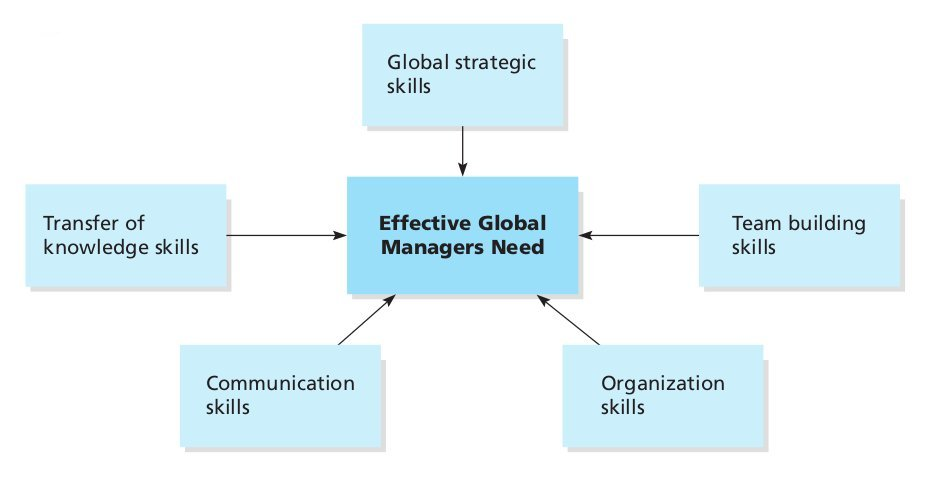
\includegraphics[scale=0.3]{"./image/Skills/Managerial Skills for the Global Marketplace.jpg"}
	\end{minipage}
	\caption{Competências de Gestão. \cite{book_6}}
\end{figure}






\begin{comment}
a) Realizar um diagnóstico de competências pessoais;\\
b) Definir objetivos de carreira;\\
c) Definir as competências que considere que no futuro lhe permitirão atingir os referidos objetivos;\\
d) Definir um plano de desenvolvimento para as competências anteriormente selecionadas.
\end{comment}\\ \\


\begin{comment}
que o aluno considere

fundamentais no contexto do trabalho do futuro, para atingir os seus objetivos
profissionais. Para tal, deverá:
a) Realizar um diagnóstico de competências pessoais;
b) Definir objetivos de carreira;
c) Definir as competências que considere que no futuro lhe permitirão atingir os
referidos objetivos;
d) Definir um plano de desenvolvimento para as competências anteriormente
selecionadas.
• A componente individual do trabalho a realizar por cada aluno deverá ser entregue em forma de um padlet (https://padlet.com) que demonstre todas as pesquisas e inputs a que o aluno recorreu para a realização do trabalho bem como as suas reflexões. O padlet deve terminar com a apresentação do plano de
desenvolvimento pessoal de competências.
• Cada aluno deverá defender oralmente a componente individual.
\end{comment}

\newpage
\section{Conclusão}
%%%%%%%%%%%%%%%%%%%%%%%%%%%%%%%%%%%%%%%%%%%%%%%%%%%%%%%%%%%%%%%%%



%%%%%%%%%%%%%%%%%%%%%%%%%%%%%%%%%%%%%%%%%%%%%%%%%%%%%%%%%%%%%%%%%
\newpage
%%%%%%%%%%%%%%%%%%%%%%%%%%
%\part*{Equa\c{c}\~{o}es} \label{eq}
%
\begin{flushleft}
{\bf Corrente Continua Condi\c{c}\~{o}es \index{Condi\c{c}\~{o}es} iniciais \index{iniciais} nulas \index{nulas}.}\par
\end{flushleft}
 \quad Circuito \index{Circuito} $LC$ em $C.C$:\par
%
\begin{itemize}
\item
$i(t)=\frac{V_{DC}\sqrt{LC}}{L}\quad \sin \left( \frac{t}{\sqrt{LC}}\right)\times u(t)$\par
\item
$V_L(t)=V_{DC}\quad \cos\left(\frac{t}{\sqrt{LC}} \right)\times u(t)$\par
\item
$V_c(t)=V_{DC}\quad \left(1-\cos\left(\frac{t}{\sqrt{LC}} \right) \right)\times u(t)$\par
\item
$\omega_n=\frac{1}{\sqrt{LC}}$\par
\item
$\overline{Z}=\sqrt{(\omega_n L-\frac{1}{\omega_n C})^2}$\par
\item
$\phi_p=\frac{\pi}{2}$\par
porque, $\sin(\omega_n t)= \cos(\omega_n t - \pi/2)$\par
\item
$\tau=\infty$\par
\end{itemize}
%
%%%%%%%%%%%%%%%%%%%%%
\quad Circuito \index{Circuito} $RLC$ em $C.C$:\par
%
\begin{enumerate}
%enum1
\item
Para \quad $C(C R^2-4 L)>0$ \quad (Ra\'{i}zes \index{Ra\'{i}zes} reais \index{reais} diferentes \index{diferentes}) \quad Sobreamortecido \index{Sobreamortecido}.\par
%
\begin{itemize}
\item
$i(t)=\frac{2 V_{DC} C e^{\frac{-tR}{2L}} sinh \left( \frac{t \sqrt{C(CR^2-4L)}}{2CL} \right)}{\sqrt{C(CR^2-RL)}}\times u(t)$\par
\item
$V_R(t)=R\times i(t)$\par
\item
$V_L(t)=L\dfrac{di(t)}{dt}$\par
%
\begin{minipage}{0.95\linewidth}
\makebox[\linewidth]{
\includegraphics[scale=0.75]{./Image/equacoes_1.png}
}
\end{minipage}\par
%
\item
$V_C(t)=\frac{1}{C}\int_0^ti(t)$\par
%
\begin{minipage}{0.95\linewidth}
\makebox[\linewidth]{
\includegraphics[scale=0.75]{./Image/equacoes_2.png}
}
\end{minipage}\par
%
\end{itemize}
%enum2
\item
Para \quad $C(C R^2-4 L)=0$ \quad (Ra\'{i}zes \index{Ra\'{i}zes} iguais \index{iguais})\quad Amortecimento \index{Amortecimento} cr\'{i}tico \index{cr\'{i}tico}.\par
%
\begin{itemize}
\item
$i(t)=\frac{V_{DC}}{L} \quad  t \quad e^{\frac{-R t}{2L}} \times u(t)$\par
\item
$V_R(t)=R\times i(t)$\par
\item
$V_L(t)=L\dfrac{di(t)}{dt}$\par
%
\begin{minipage}{0.95\linewidth}
\makebox[\linewidth]{
\includegraphics[scale=0.75]{./Image/equacoes_3.png}
}
\end{minipage}\par
%
\item
$V_C(t)=\frac{1}{C}\int_0^ti(t)$\par
\begin{minipage}{0.95\linewidth}
\makebox[\linewidth]{
\includegraphics[scale=0.75]{./Image/equacoes_4.png}
}
\end{minipage}\par
%
\end{itemize}
%enum3
\item
Para \quad $C(C R^2-4 L)<0$ \quad (Ra\'{i}zes \index{Ra\'{i}zes} complexas \index{complexas}) \quad Amortecido \index{Amortecido}.\par
%
\begin{itemize}
\item
$i(t)=\frac{2 V_{DC} C e^{\frac{-tR}{2L}} sin \left( \frac{t \sqrt{-C(CR^2-4L)}}{2CL} \right)}{\sqrt{-C(CR^2-4L)}}\times u(t)$\par
\item
$V_R(t)=R\times i(t)$\par
\item
$V_L(t)=L\dfrac{di(t)}{dt}$\par
%
\begin{minipage}{0.95\linewidth}
\makebox[\linewidth]{
\includegraphics[scale=0.75]{./Image/equacoes_5.png}
}
\end{minipage}\par
%
\item
$V_C(t)=\frac{1}{C}\int_0^ti(t)$\par
%
\begin{minipage}{0.95\linewidth}
\makebox[\linewidth]{
\includegraphics[scale=0.75]{./Image/equacoes_6.png}
}
\end{minipage}\par
%
\end{itemize}
\end{enumerate}
%
\begin{itemize}
\item
$| \omega_n |=\sqrt{\frac{4 L-R^2 C}{4 L^2 C}}$\par
\item
%\overrightarrow{Z}
$\overline{Z}=\sqrt{R^2 + (\omega_n L -\frac{1}{\omega_n C})^2}$\par
\item
$\phi_p=\arctan\left(\frac{\omega_n L - \frac{1}{\omega_n C}}{R}\right)$\par
\item
$\tau=\frac{2 L}{R}$\par
\end{itemize}
%%%%%%%%%%%%%%%%%%%%%%%%%%%%%%%%%%%%%%%%%%
\begin{flushleft}
{\bf Corrente \index{Corrente} Alternada condi\c{c}\~{o}es \index{Condi\c{c}\~{o}es} iniciais \index{iniciais} nulas \index{nulas}}.
\end{flushleft}
\quad Circuito \index{Circuito} $RLE$ em $C.A$:\par
\begin{itemize}
\item
$i(t)=C_T\ e^{-\frac{R}{L}t}+\frac{V_{m\acute{a}x}}{\overline{Z}}\sin(\omega t + \alpha - \phi_p)-\frac{E}{R}$\newline
$i(t)=C_T\ e^{-\frac{R}{L}t} + C_1 \cos (\omega t) + C_2 \sin(\omega t)-\frac{E}{R}$
\item
$I(\omega t)=C_T\ e^{-\frac{R}{L \omega}\omega t}+\frac{V_{m\acute{a}x}}{\overline{Z}}\sin(\omega t + \alpha - \phi_p)-\frac{E}{R}$
\item
$\overrightarrow{Z}=R+j\omega L$\\
$\overline{Z}=\sqrt{R^2 + (\omega L)^2}$
\item
$\phi_p=\arctan(\frac{\omega L}{R})$
\item
$C_T=\frac{E}{R}-\frac{V_{m\acute{a}x}}{\overline{Z}}\sin(\alpha - \phi_p)$
\item
$C_T=\frac{V_{m\acute{a}x}}{R^2 + (\omega L)^2}(L \omega \cos(\alpha) - R \sin (\alpha))+\frac{E}{R}$
\item
$C_1=\frac{V_{m\acute{a}x}}{R^2 + (\omega L)^2}(R \sin (\alpha) - L \omega \cos(\alpha))$
\item
$C_2=\frac{V_{m\acute{a}x}}{R^2 + (\omega L)^2}(R \cos (\alpha) + L \omega \sin (\alpha))$
%
\end{itemize}
%%%%%%%%%%%%%%%%%%%%%%%
%\part*{Defini\c{c}\~{o}es} \label{def}
\begin{definition}
Capacit\^{a}ncia
\begin{flalign*}
Q_c(t) =& \int^t i(t) \quad dt & \\
=& Q_c(0^-)+\int_{0^-}^t i(t) \quad dt & \\
V_c(t) =& \frac{Q_c(t)}{C} & \\
=& \frac{1}{C} \quad \int^t i_c(t) \quad dt & \\
=& \frac{Q_c(0^-)}{C} + \frac{1}{c} \quad \int_0^t i_c(t) \quad dt & \\
=& V(0^-) + \frac{1}{c} \quad \int_0^t i_c(t) \quad dt & \\
i_c(t) =& C \quad \dfrac{d V_c(t)}{dt} &
\end{flalign*}\par
\end{definition}
%
\begin{definition}
Indut\^{a}ncia
\begin{flalign*}
\psi_L(t) =& \int^t V_L(t) \quad dt & \\
=& \psi_L(0^-)+\int_{0^-}^t V_L(t) \quad dt & \\
V_L(t) =& L \quad \dfrac{d i_L(t)}{dt} & \\
i_L(t) =& \frac{\psi_L(t)}{L} & \\
=& \frac{1}{L} \quad \int^t V_L(t) \quad dt & \\
=& \frac{\psi_L(0^-)}{L} + \frac{1}{L} \quad \int_0^t V_L(t) \quad dt & \\
=& i_L(0^-) + \frac{1}{L} \quad \int_0^t V_L(t) \quad dt &
\end{flalign*}\par
\end{definition}
%
\begin{definition}
Resist\^{e}ncia
\begin{flalign*}
V_R(t) =& R \quad i_R(t) & \\
i_R(t) =& \frac{V_R(t)}{R} &
\end{flalign*}\par
\end{definition}
%
\begin{definition}
Valor M\'{e}dio
\begin{flalign*}
X_{av} =& \frac{1}{T} \; \int_0^T X(t) dt &
\end{flalign*}\par
\end{definition}
%
\begin{definition}
Valor Eficaz
\begin{flalign*}
X_{ef} =& \sqrt{ \frac{1}{T} \; \int_0^T \overset{\text{2}}{X(t)} dt } &
\end{flalign*}\par
\end{definition}
%

%%%%%%%%%%%%%%%%%%%%%%%%%%
%Figuras Bibliografia Index
\listoffigures
\cite{*}
\bibliography{./bibliography/Bibliography}
%\printindex
\newpage
\footnote{Apontamento}
\end{document}
%%%%%%%%%%%%%%%%%%%%%%%%%%%%%%%%%%%%%%%%%%%%%%%%%%%%%%%%%%%%%%%%%
\begin{comment}
Vamos montar uma empresa, eu monto e tu vais ser a empresa. \\
Um palerma nasce a cada minuto.\\
No futuro existe um grau elevado de incerteza, com muitos problemas pelo caminho, a solução para os problemas tem duas soluções, ou fazer nada, na qual tem duas saídas, ou fica estático, isto é igual mas com um grande grau de probabilidade de piorar, a outra alternativa é fazer mudanças, seja qual for e esperar o resultado, caso negativo mudar novamente de direção desde que não seja a mesma, a rapidez de este processo tem uma grande esperança de garantia de sucesso, no entanto haverá casos de problemas já reconhecidos e os remédios também, dando um avanço e vantagem a nível de competição, isto requer sabedoria e conhecimentos adquiridos das velhas gerações.\\
Existe a preocupação da desigualdade da distribuição da riqueza sendo que a procura vai estar mais centrada a volta de competências tecnológicas e existir disparidade salarial entre as classes trabalhadoras, no entanto Portugal vive numa cultura antitético a estas mudanças com lideres totalmente desligados e desatualizados, e quando o país atravessa situações de calamidade a solidariedade são suas únicas formas de luta.\\
\end{comment}
%%%%%%%%%%%%%%%%%%%%%%%%%%%%%%%%%%%%%%%%%%%%%%%%%%%%%%%%%%%%%%%%%